\chapter{Druck, freie Energie und Energieschwankungen}

\lectureoverview{Wir leiten den Druck aus der Zustandssumme her, ohne ein kinetisches Bild von Molekülen vorauszusetzen, die gegen eine Wand stoßen. Ein geometrisches Lemma überführt eine adiabatische Ableitung in Ableitungen bei fester Temperatur, die Helmholtz freie Energie stellt die Verbindung zu \(\log Z\) her, und als erste Anwendung ergibt sich das ideale Gasgesetz. Anschließend leiten wir mit derselben Zustandssumme die Energiefluktuation im Gleichgewicht und ihren Zusammenhang mit der Wärmekapazität her.}

\section{Die Mathematik soll die Intuition prüfen}

Die Thermodynamik hat einen eigenartigen Ruf. Ihre Analysis ist elementar, doch die Wahl dessen, was man ableitet und konstant hält, kann ausgesprochen subtil sein. Unsere Fragestellung ist bewusst eng gefasst: Wir berechnen den Druck eines idealen Gases. Der Weg zu dieser Antwort soll jedoch allgemein genug sein, um auch für Systeme zu gelten, in denen das vertraute Bild der Moleküle nicht mehr zuverlässig ist.

Die kinetische Erklärung ist leicht zu erzählen. Moleküle stoßen gegen eine Wand und kehren die Normalkomponente ihres Impulses um. Der pro Zeiteinheit übertragene Impuls ergibt die Kraft, und die Kraft pro Flächeneinheit den Druck. Wir wissen bereits, dass die mittlere kinetische Energie pro Molekül in drei Dimensionen \begin{equation}
 \left\langle \frac{p^2}{2m}\right\rangle=\frac{3}{2}T
 \qquad (k_B=1).
 \label{eq:sm5-mean-kinetic-energy}
\end{equation} beträgt. Mit einer isotropen Geschwindigkeitsverteilung lassen sich die Stoßrate, der Impulsübertrag bei jedem Stoß und der daraus folgende Druck abschätzen.

Doch die Wand selbst scheint die Isotropie zu stören. Warum sollten Moleküle unmittelbar an der Begrenzung dieselbe Verteilung von Geschwindigkeiten und Richtungen haben wie Moleküle tief im Inneren? Im Gleichgewicht ist das, soweit es hier relevant ist, tatsächlich der Fall. Diese Schlussfolgerung sollte sich jedoch aus der statistischen Mechanik ergeben, statt als Intuition in die Rechnung eingeschleust zu werden. Stöße zwischen den Molekülen machen das kinetische Argument noch undurchsichtiger. Das nicht wechselwirkende Gas ist gerade deshalb leicht zu behandeln, weil es ein ungewöhnlich einfaches System ist.

In der Physik gibt es Situationen, in denen es am sichersten ist, das anschauliche Bild vorübergehend zurückzustellen und der Mathematik zu folgen. Man bestimmt die gesuchte Größe, formt die allgemeinen Beziehungen um und wartet, bis eine wiedererkennbare Formel erscheint. Am Ende kehrt die Intuition zurück; dann prüft aber die Mathematik die Intuition und nicht umgekehrt. Der Reiz der Thermodynamik liegt in den überraschenden Beziehungen, die aus diesem Vorgehen hervorgehen.

Gesucht ist eine Zustandsgleichung, \begin{equation}
 P=P(T,V,N),
 \label{eq:sm5-equation-of-state-target}
\end{equation} wobei \(N\) die Stoffmenge, \(T\) die Temperatur und \(V\) das Volumen bezeichnet. Eine überzeugende Herleitung sollte auch dann sinnvoll bleiben, wenn die Teilchen miteinander wechselwirken oder der Stoff eine Flüssigkeit, ein Plasma oder ein Festkörper ist. Erst die abschließende Auswertung der Zustandssumme wird auf ein ideales Gas spezialisiert.

\section{Entropie und Helmholtz freie Energie}

Rufen wir zunächst die kanonischen Formeln ab, die wir später benötigen. Für Mikrozustände mit den Bezeichnungen \(i\) gilt \begin{equation}
 \begin{aligned}
 S&=-\sum_i p_i\log p_i,\\
 p_i&=\frac{e^{-\beta E_i}}{Z},\\
 Z&=\sum_i e^{-\beta E_i}.
 \end{aligned}
 \label{eq:sm5-canonical-definitions}
\end{equation} Der Logarithmus der Wahrscheinlichkeit lautet \begin{equation}
 \log p_i=-\beta E_i-\log Z.
 \label{eq:sm5-log-probability}
\end{equation}. Eingesetzt in die Entropie ergibt sich \begin{align}
 S
 &=-\sum_i p_i\log p_i \notag\\
 &=\beta\sum_i p_iE_i+\log Z\sum_i p_i \notag\\
 &=\beta E+\log Z.
 \label{eq:sm5-entropy-log-z}
\end{align}. Hier ist \(E=\sum_i p_iE_i\) die mittlere Energie.

\begin{classroomqa}\audiencequestion{Warum ergibt der zweite Term nur \(\log Z\) und nicht die Anzahl der Zustände mal \(\log Z\)?}\lecturerresponse{Der aufsummierte Koeffizient ist \(p_i\), nicht \(1\). Aus der Normierung folgt \(\sum_i p_i=1\). Gleichwertig dazu kürzt sich der Zähler \(\sum_i e^{-\beta E_i}=Z\) mit dem \(Z\) im Nenner. Die Anzahl der Zustände kommt in diesem Schritt nicht vor.\lecturetimestamp{00:14:25--00:14:55}}\end{classroomqa}

In den Energieeinheiten, die im größten Teil der Vorlesung verwendet werden, gilt \(\beta=1/T\). Multipliziert man \eqref{eq:sm5-entropy-log-z} mit \(T\) und formt um, erhält man \begin{equation}
 E-TS=-T\log Z.
 \label{eq:sm5-helmholtz-identity}
\end{equation}. Die linke Seite dieser Gleichung tritt so häufig auf, dass sie einen eigenen Namen verdient: \begin{equation}
 A\equiv E-TS,
 \qquad
 A=-T\log Z.
 \label{eq:sm5-helmholtz-definition}
\end{equation}. Das ist die Helmholtz freie Energie. Im Moment ist der Name weniger wichtig als die Identität selbst; wir werden sie benötigen, um den Druck in eine Ableitung der Zustandssumme umzuwandeln.

\begin{figure}[t]\centering
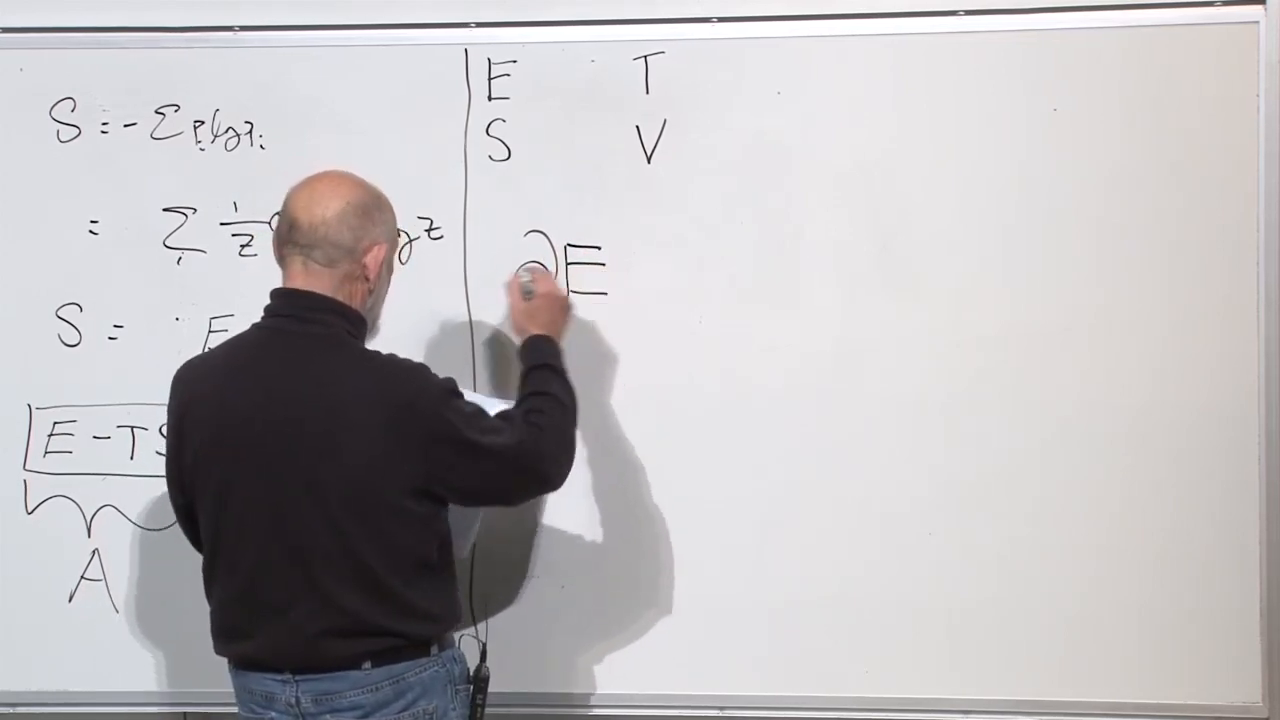
\includegraphics[width=0.90\textwidth]{lecture_05_figure_03.png}\caption{\(A=E-TS=-T\log Z\)}\lectureframe{00:16:50}\end{figure}

\section{Kontrollparameter und ihre Antworten}

Ein Kontrollparameter ist eine makroskopische Größe, die sich von außen durch einen Experimentator verändern lässt. Eine Verschiebung des Kolbens ändert das Volumen, ohne dass einzelne Moleküle manipuliert werden müssen. Angelegte elektrische und magnetische Felder sind weitere Beispiele. In einem allgemeineren Ensemble kann auch die Teilchenzahl variabel sein.

Thermodynamische Variablen treten natürlicherweise in konjugierten Paaren auf. Im vorliegenden Problem ist das Volumen der Kontrollparameter und der Druck seine Antwort. Wir verändern \(V\); der Druck gibt an, wie stark sich das System energetisch gegen diese Änderung wehrt. Später wird die Ableitung der Energie diese Paarung präzisieren.

\begin{classroomqa}\audiencequestion{Kann man den Druck selbst als Kontrollparameter auffassen?}\lecturerresponse{Man kann ein Experiment so gestalten, dass der äußere Druck festgelegt wird. Bei der hier betrachteten Anordnung legt jedoch die Kolbenposition das Volumen fest, und der Innendruck ist die Antwort des Systems. Druck und Volumen sind konjugierte Variablen; welche davon kontrolliert wird, hängt vom Ensemble und vom Versuchsaufbau ab.\lecturetimestamp{00:19:22--00:20:01}}\end{classroomqa}

\begin{classroomqa}\audiencequestion{Wird angenommen, dass alle Moleküle identisch sind, oder ist das Argument auf ein Gas beschränkt?}\lecturerresponse{Für das thermodynamische Argument ist keine solche Einschränkung nötig. Der Zylinder kann mehrere Teilchensorten, eine Flüssigkeit oder sogar einen komprimierten Festkörper enthalten. Erst nachdem die allgemeine Druckformel hergeleitet wurde, dient die Zustandssumme des idealen Gases als Spezialanwendung.\lecturetimestamp{00:20:02--00:20:39}}\end{classroomqa}

\begin{classroomqa}\audiencequestion{Könnte man die Stoffmenge durch einen weiteren äußeren Eingriff verändern?}\lecturerresponse{Ja. Die Teilchenzahl ist ein weiterer möglicher Kontrollparameter. Behandelt man sie als veränderlich, gehört dazu eine eigene konjugierte Variable: das chemische Potenzial. Für die Rechnung heute Abend bleibt \(N\) fest.\lecturetimestamp{00:20:39--00:20:57}}\end{classroomqa}

\begin{classroomqa}\audiencequestion{Können flüssiges Wasser und Dampf gleichzeitig im Gleichgewicht vorliegen?}\lecturerresponse{Bei der Koexistenztemperatur und dem Koexistenzdruck können sie das. Die Schwerkraft kann die Flüssigkeit unterhalb des Dampfes anordnen; dennoch können beide Phasen dieselbe Temperatur haben und sich im thermischen Gleichgewicht befinden. Derselbe allgemeine statistisch-mechanische Rahmen gilt auch hier.\lecturetimestamp{00:20:59--00:21:36}}\end{classroomqa}

Betrachten wir für das nächste Argument Energie und Entropie als abhängige Funktionen zweier unabhängig einstellbarer Variablen: \begin{equation}
 E=E(T,V),
 \qquad
 S=S(T,V).
 \label{eq:sm5-dependent-functions}
\end{equation}. Temperatur und Volumen bilden Koordinaten im thermodynamischen Zustandsraum. Energie und Entropie ordnen jedem Gleichgewichtspunkt in diesem Raum jeweils eine Zahl zu.

\section{Die Ableitung bei konstanter Entropie}

Die Ableitung, die wir letztlich benötigen, ist ungewöhnlich: \[
 \left(\frac{\partial E}{\partial V}\right)_S.
\]. Obwohl \(T\) und \(V\) die unabhängigen Koordinaten sind, wird bei dieser Ableitung \(V\) verändert, während die abhängige Funktion \(S(T,V)\) konstant gehalten wird. Es handelt sich um eine Ableitung entlang einer Kurve in der \((T,V)\)-Ebene, nicht entlang einer Koordinatenachse.

\begin{classroomqa}\audiencequestion{Wie können \(T\) und \(V\) unabhängig sein, wenn später die Ableitung \(dT/dV\) verwendet wird?}\lecturerresponse{Im gesamten Zustandsraum sind sie unabhängig. Sobald wir die Bedingung \(S(T,V)=\mathrm{constant}\) auferlegen, liegen die zulässigen Zustände auf einer eindimensionalen Kontur. Entlang dieser Kontur wird \(T\) zu einer Funktion von \(V\), und ihre Steigung \(dT/dV\) ist wohldefiniert.\lecturetimestamp{01:01:18--01:02:09}}\end{classroomqa}

\begin{lemma}Wenn \(E(T,V)\) und \(S(T,V)\) differenzierbar sind, gilt überall dort, wo \((\partial S/\partial T)_V\neq0\), \begin{equation}
 \left(\frac{\partial E}{\partial V}\right)_S
 =
 \left(\frac{\partial E}{\partial V}\right)_T
 -
 \left(\frac{\partial E}{\partial S}\right)_V
 \left(\frac{\partial S}{\partial V}\right)_T.
 \label{eq:sm5-calculus-lemma}
\end{equation}\end{lemma}

\begin{proof}Für eine beliebige infinitesimale Verschiebung gilt \begin{equation}
 dE=
 \left(\frac{\partial E}{\partial V}\right)_T dV
 +
 \left(\frac{\partial E}{\partial T}\right)_V dT.
 \label{eq:sm5-total-differential-e}
\end{equation}. Bei festem \(V\) erlaubt die Kettenregel, \(S\) als Zwischenvariable zu verwenden: \begin{equation}
 \left(\frac{\partial E}{\partial T}\right)_V
 =
 \left(\frac{\partial E}{\partial S}\right)_V
 \left(\frac{\partial S}{\partial T}\right)_V.
 \label{eq:sm5-chain-rule-e-s-t}
\end{equation}

Beschränken wir die Verschiebung nun auf eine Kontur, auf der \(S\) konstant ist. Entlang dieser Kontur gilt \begin{equation}
 0=dS=
 \left(\frac{\partial S}{\partial V}\right)_T dV
 +
 \left(\frac{\partial S}{\partial T}\right)_V dT.
 \label{eq:sm5-constant-entropy-differential}
\end{equation}. Auflösen nach der Steigung der Kontur ergibt \begin{equation}
 \left(\frac{dT}{dV}\right)_S
 =
 -
 \frac{\left(\frac{\partial S}{\partial V}\right)_T}
 {\left(\frac{\partial S}{\partial T}\right)_V}.
 \label{eq:sm5-entropy-contour-slope}
\end{equation}. Teilen wir \eqref{eq:sm5-total-differential-e} durch \(dV\), verwenden \eqref{eq:sm5-chain-rule-e-s-t} und setzen \eqref{eq:sm5-entropy-contour-slope} ein, so folgt \begin{align}
 \left(\frac{\partial E}{\partial V}\right)_S
 &=
 \left(\frac{\partial E}{\partial V}\right)_T
 +
 \left(\frac{\partial E}{\partial S}\right)_V
 \left(\frac{\partial S}{\partial T}\right)_V
 \left(\frac{dT}{dV}\right)_S \notag\\
 &=
 \left(\frac{\partial E}{\partial V}\right)_T
 -
 \left(\frac{\partial E}{\partial S}\right)_V
 \left(\frac{\partial S}{\partial V}\right)_T.
\end{align}. Der Faktor \((\partial S/\partial T)_V\) hat sich herausgekürzt; damit ist das Ergebnis bewiesen.\end{proof}

\begin{figure}[t]\centering
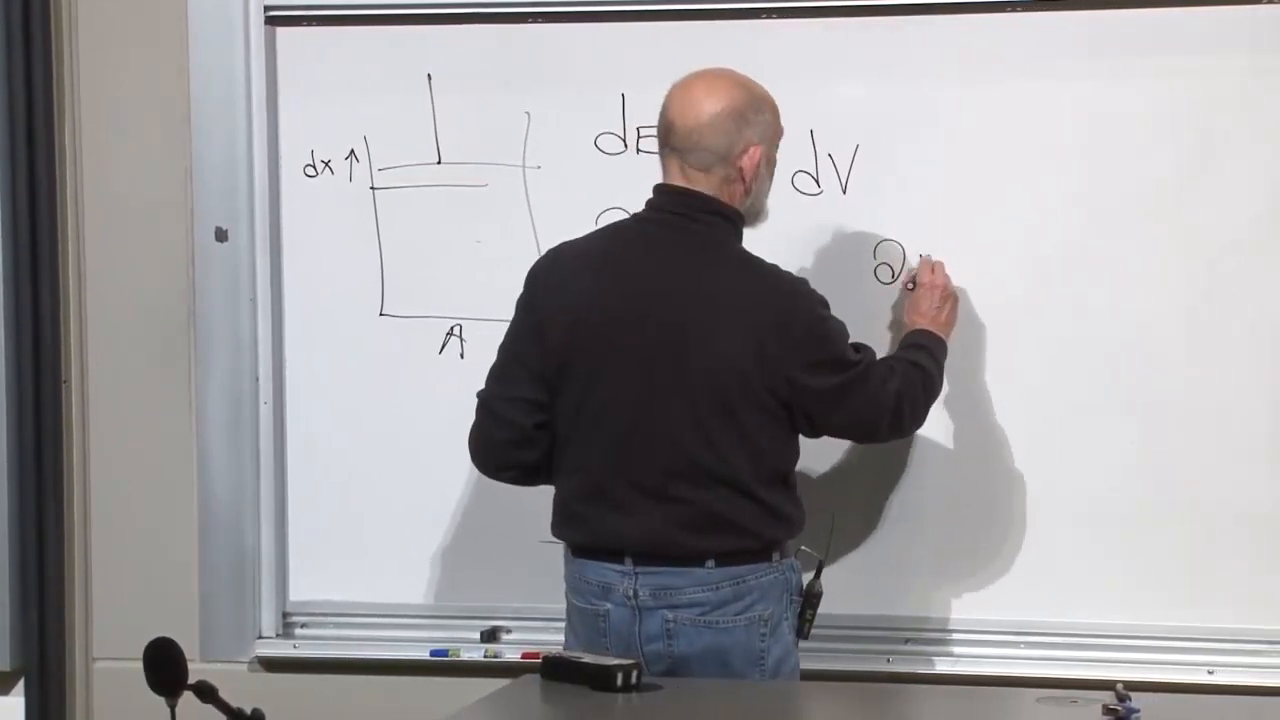
\includegraphics[width=0.90\textwidth]{lecture_05_figure_04.png}\caption{Die Berechnung entlang der Kontur konstanter Entropie an dem Punkt, an dem sich der Faktor herauskürzt und das Ableitungslemma damit bewiesen ist.}\lectureframe{00:36:10}\end{figure}

Das geometrische Bild ist keine bloße Zierde. Es erklärt, warum sich eine scheinbar ungewöhnliche Ableitung bei festem \(S\) mit gewöhnlichen partiellen Ableitungen nach den unabhängigen Koordinaten \(T\) und \(V\) berechnen lässt. Während der Herleitung \(\delta E/\delta V\) zu schreiben, erinnert daran, dass die Symbole Verhältnisse kleiner Änderungen entlang eines festgelegten Weges darstellen.

\begin{classroomqa}\audiencequestion{Ist die Entwicklung von \(dE\) einfach die übliche Definition partieller Ableitungen?}\lecturerresponse{Ja. Im totalen Differential ist nichts Besonderes enthalten. Hinzu kommt nur die spätere Einschränkung auf die Kontur \(dS=0\), die den Zusammenhang zwischen \(dT\) und \(dV\) festlegt.\lecturetimestamp{00:29:26--00:29:32}}\end{classroomqa}

\begin{classroomqa}\audiencequestion{Muss für die Kürzung \((\partial S/\partial T)_V\) von null verschieden sein?}\lecturerresponse{Ja. Für ein gewöhnliches stabiles System gilt \[
 \left(\frac{\partial S}{\partial T}\right)_V
 =\frac{C_V}{T}>0,
\], sodass die Division zulässig ist. In Ausnahmefällen ist eine gesonderte Betrachtung nötig. Bei festem Hamiltonoperator verbreitert eine Temperaturerhöhung die kanonische Energieverteilung und erhöht gewöhnlich die Entropie; eine Temperaturerniedrigung verengt sie. Das ist die physikalisch richtige Richtung des Monotoniearguments.\lecturetimestamp{00:36:50--00:37:47}}\end{classroomqa}

\section{Kolbenarbeit und adiabatische Bedingung}

Nun geben wir der Ableitung eine physikalische Bedeutung. Betrachten wir einen Kolben mit der Querschnittsfläche \(\mathcal A\). Bewegt er sich um \(dx\) nach außen, gilt \begin{equation}
 dV=\mathcal A\,dx.
 \label{eq:sm5-piston-volume}
\end{equation}. Das Gas übt die Kraft \(P\mathcal A\) auf den Kolben aus. Die vom Gas verrichtete Arbeit ist daher \begin{equation}
 \delta W_{\mathrm{by}}=P\mathcal A\,dx=P\,dV.
 \label{eq:sm5-piston-work}
\end{equation}. Tritt keine Wärme in das Gas ein, folgt aus der Energieerhaltung \begin{equation}
 dE=-P\,dV.
 \label{eq:sm5-adiabatic-work}
\end{equation}. Das Vorzeichen hat eine physikalische Bedeutung: Bei der Expansion hebt das Gas den Kolben an oder beschleunigt ihn, und seine eigene Energie nimmt ab.

\begin{figure}[t]\centering
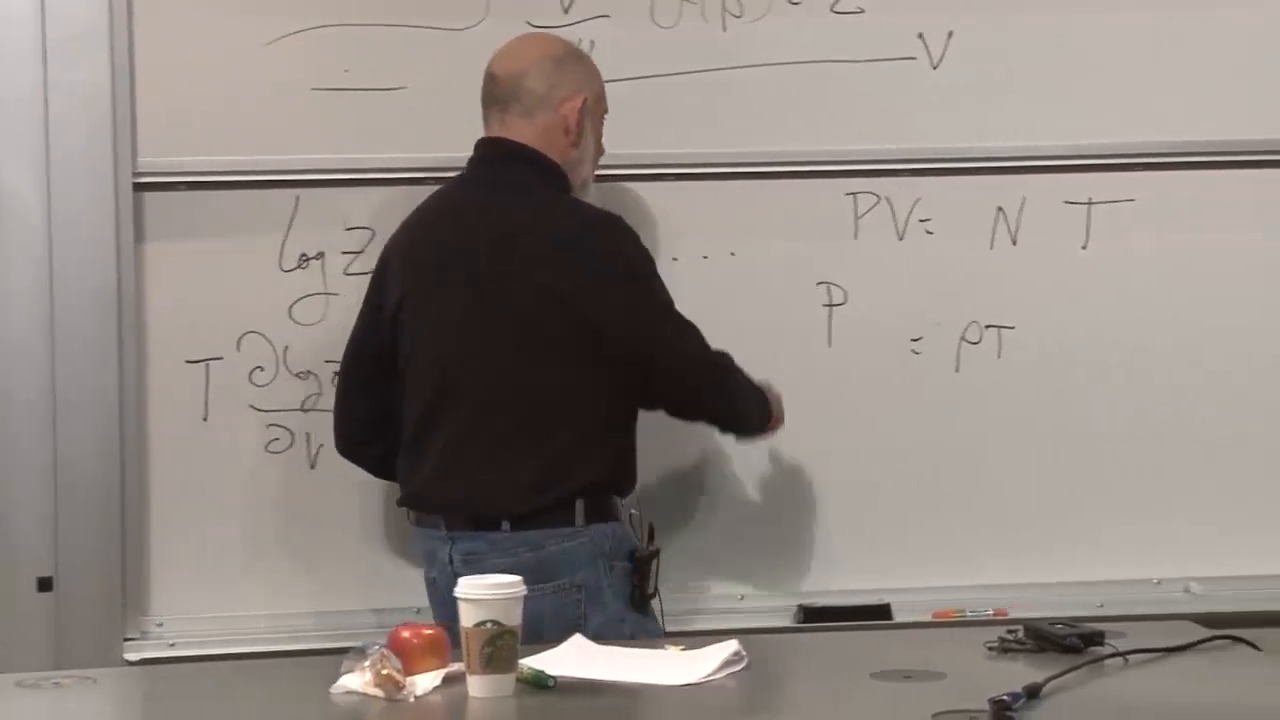
\includegraphics[width=0.90\textwidth]{lecture_05_figure_05.png}\caption{Die Geometrie des Kolbens und die vollständige Arbeitsbeziehung \(dE=-P\,dV\).}\lectureframe{00:43:10}\end{figure}

Zwei Einschränkungen sind wesentlich. Der Kolben muss sich langsam genug bewegen, damit das System beliebig nahe am Gleichgewicht bleibt, und die Wände müssen isoliert sein, damit keine Energie in Form von Wärme zugeführt wird. Ein schneller Zug kann so rasch erfolgen, dass während der Bewegung kein Molekül den zurückweichenden Kolben erreicht. Eine schnelle Kompression löst Stoßwellen aus. Keiner dieser Vorgänge lässt sich als Folge von Gleichgewichtszuständen darstellen.

Das Wort \emph{adiabatisch} wird bisweilen für fehlenden Wärmeaustausch und bisweilen für eine langsame Änderung verwendet. Beim hier erforderlichen reversiblen Vorgang spielen beide Bedeutungen eine Rolle: Die Änderung verläuft quasistatisch und das System ist thermisch isoliert. Unter diesen Bedingungen ist sie zugleich isentrop.

\begin{classroomqa}\audiencequestion{Warum bleibt die Entropie bei einer adiabatischen Änderung konstant?}\lecturerresponse{Betrachten wir das System quantenmechanisch. Seine Vielteilchenenergieniveaus hängen vom Volumen ab. Ändert sich \(V\) langsam, führt der adiabatische Satz jedes besetzte Niveau stetig in sein Nachfolgeniveau über, ohne Übergänge zwischen den Niveauindizes. Die Energien \(E_i(V)\) ändern sich, die Besetzungswahrscheinlichkeiten \(p_i\) bleiben jedoch unverändert. Da \(S=-\sum_i p_i\log p_i\) von diesen Wahrscheinlichkeiten abhängt, bleibt auch die Entropie konstant. Wärmeaustausch oder irreversible Bewegung würden diese Schlussfolgerung ungültig machen.\lecturetimestamp{00:43:37--00:49:15}}\end{classroomqa}

\begin{figure}[t]\centering
\includegraphics[width=0.90\textwidth]{lecture_05_figure_06.png}\caption{Vielteilchenenergieniveaus verschieben sich mit dem Volumen, während ihre Besetzungswahrscheinlichkeiten den jeweiligen Niveauindizes zugeordnet bleiben.}\lectureframe{00:48:50}\end{figure}

Gleichung \eqref{eq:sm5-adiabatic-work}, ausgewertet entlang dieses Weges konstanter Entropie, weist den Druck aus als \begin{equation}
 P=-\left(\frac{\partial E}{\partial V}\right)_S.
 \label{eq:sm5-pressure-fixed-entropy}
\end{equation}. Das ist die konjugierte Beziehung zwischen Druck und Volumen.

\begin{classroomqa}\audiencequestion{Was passiert, wenn der Kolben stattdessen schnell bewegt wird?}\lecturerresponse{Das System verlässt das Gleichgewicht, und seine detaillierte Dynamik wird wichtig. Eine plötzliche Kompression erzeugt einen Stoß. Bei einer idealen freien Expansion kann sich der Kolben zurückziehen, bevor ihn ein Molekül trifft; dann wird keine Arbeit verrichtet und die Energie bleibt konstant, obwohl sich das Volumen ändert. Das Gas stellt später unter Zunahme der Entropie das Gleichgewicht wieder her. Solche Vorgänge lassen sich nicht mit der einzelnen Gleichgewichtsableitung in \eqref{eq:sm5-pressure-fixed-entropy} beschreiben.\lecturetimestamp{00:58:30--01:01:15}}\end{classroomqa}

\begin{classroomqa}\audiencequestion{Welche quantitative Bedingung entscheidet, ob eine Änderung langsam ist?}\lecturerresponse{Die Zeit, über die sich die äußeren Bedingungen ändern, muss groß sein im Vergleich zu den relevanten inneren Relaxationszeiten. Bei einem Gas sollten während der makroskopischen Änderung viele Molekülstöße und viele Stöße gegen die Wände stattfinden. Die genaue Zeitskala hängt vom Material und von der Geometrie ab; der quasistatische Grenzfall ist dagegen allgemein.\lecturetimestamp{01:02:09--01:03:20}}\end{classroomqa}

\section{Von der adiabatischen Energie zur Zustandssumme}

Die physikalische Formel \eqref{eq:sm5-pressure-fixed-entropy} ist noch nicht diejenige, die sich am einfachsten berechnen lässt. Die kanonische statistische Mechanik liefert auf natürliche Weise Funktionen der Temperatur, denn \(T\) tritt unmittelbar im Boltzmann-Faktor auf. Das Analysislemma überführt die unhandliche Ableitung bei konstanter Entropie in diese für Berechnungen geeignete Form: \begin{align}
 P
 &=
 -\left(\frac{\partial E}{\partial V}\right)_T
 +
 \left(\frac{\partial E}{\partial S}\right)_V
 \left(\frac{\partial S}{\partial V}\right)_T.
 \label{eq:sm5-pressure-lemma-substitution}
\end{align}. Bei festem Volumen liefert der erste Hauptsatz \(dE=T\,dS\) und damit \begin{equation}
 \left(\frac{\partial E}{\partial S}\right)_V=T.
 \label{eq:sm5-e-s-temperature}
\end{equation}. Somit gilt \begin{equation}
 P=
 -\left(\frac{\partial E}{\partial V}\right)_T
 +
 T\left(\frac{\partial S}{\partial V}\right)_T.
 \label{eq:sm5-pressure-fixed-temperature-pieces}
\end{equation}

\begin{classroomqa}\audiencequestion{Woher kommt das Minuszeichen in der Druckformel?}\lecturerresponse{Es stammt aus der vom Gas verrichteten Arbeit: \(dE=-P\,dV\) bei adiabatischer Expansion. Das Analysislemma selbst enthält zwischen seinen beiden Termen ein Minuszeichen; das vorangestellte Minus in \(P=-(\partial E/\partial V)_S\) kehrt beide Terme um und ergibt \eqref{eq:sm5-pressure-fixed-temperature-pieces}.\lecturetimestamp{00:52:40--00:53:14}}\end{classroomqa}

Da \(T\) in beiden Ableitungen festgehalten wird, gilt \begin{align}
 P
 &=
 -\left(\frac{\partial}{\partial V}(E-TS)\right)_T \notag\\
 &=
 -\left(\frac{\partial A}{\partial V}\right)_T.
 \label{eq:sm5-pressure-free-energy}
\end{align}. Schließlich setzen wir \(A=-T\log Z\) ein: \begin{equation}
 \boxed{
 P=
 T\left(\frac{\partial\log Z}{\partial V}\right)_T
 }.
 \label{eq:sm5-pressure-log-z}
\end{equation}

\begin{figure}[t]\centering
\includegraphics[width=0.90\textwidth]{lecture_05_figure_07.png}\caption{Die Umformung bei fester Temperatur: \(P=-(\partial A/\partial V)_T
=T(\partial\log Z/\partial V)_T\).}\lectureframe{00:55:55}\end{figure}

In \eqref{eq:sm5-pressure-log-z} wird kein ideales Gas vorausgesetzt. Lässt sich die Zustandssumme einer wechselwirkenden Flüssigkeit, eines Plasmas oder eines Festkörpers berechnen, liefert dieselbe Ableitung dessen Druck. Allgemeiner erhält man zu jedem äußeren Kontrollparameter eine konjugierte Antwortgröße, indem man ein geeignetes thermodynamisches Potenzial ableitet. Die Zustandssumme fasst viele solcher Antworten zusammen: Ableiten von \(\log Z\) nach \(\beta\) ergibt die Energie, Ableiten nach dem Volumen den Druck.

\section{Die Zustandsgleichung des idealen Gases}

Erst jetzt spezialisieren wir auf \(N\) nicht wechselwirkende Teilchen. Unter Beibehaltung der klassischen Normierung des Phasenraums gilt \begin{equation}
 Z_N=
 \frac{1}{N!h^{3N}}
 \int d^{3N}q\,d^{3N}p\,
 \exp\!\left[
 -\beta\sum_{a=1}^{N}\frac{\mathbf p_a^2}{2m}
 \right].
 \label{eq:sm5-ideal-gas-partition-integral}
\end{equation}. Es gibt \(3N\) Ortskoordinaten und \(3N\) Impulskoordinaten. Der Hamiltonoperator hängt nicht vom Ort ab, daher liefert jedes Teilchen einen Faktor, der dem Behältervolumen entspricht: \begin{equation}
 Z_N=
 \frac{V^N}{N!h^{3N}}I_p(\beta),
 \label{eq:sm5-ideal-gas-factorization}
\end{equation}, wobei das gesamte Impulsintegral \(I_p(\beta)\) unabhängig von \(V\) ist.

\begin{classroomqa}\audiencequestion{Warum gibt es \(3N\) Ortsintegrale und \(3N\) Impulsintegrale?}\lecturerresponse{Jedes der \(N\) Teilchen hat drei räumliche Koordinaten und drei konjugierte Impulskomponenten. Die Anzahl beträgt \(3N\) in jeder Hälfte des Phasenraums, nicht \(N\) Teilchen plus weitere \(3N\) Teilchen.\lecturetimestamp{01:04:19--01:04:28}}\end{classroomqa}

Ein Logarithmus trennt die Volumenabhängigkeit ab: \begin{equation}
 \log Z_N
 =
 N\log V-\log N!-3N\log h+\log I_p(\beta).
 \label{eq:sm5-log-ideal-gas-partition}
\end{equation}. Die Faktoren \(1/N!\), \(h^{-3N}\) und \(I_p(\beta)\) sind sämtlich unabhängig vom Volumen. Sie sind für die absolute Entropie und andere Fragestellungen wichtig, nicht jedoch für diese spezielle Ableitung. Daher gilt \begin{equation}
 \left(\frac{\partial\log Z_N}{\partial V}\right)_T
 =\frac{N}{V}.
 \label{eq:sm5-log-z-volume-derivative}
\end{equation}. Aus Gleichung \eqref{eq:sm5-pressure-log-z} folgt unmittelbar \begin{equation}
 P=\frac{NT}{V},
 \qquad
 \boxed{PV=NT}.
 \label{eq:sm5-ideal-gas-law}
\end{equation}

\begin{classroomqa}\audiencequestion{Zählt \(N\) weiterhin die Replikate mit, die zur Herleitung der Boltzmann-Verteilung verwendet wurden?}\lecturerresponse{Nein. Die Replikatkonstruktion war in der früheren Herleitung ein Hilfsmittel zum Zählen und kommt hier nicht mehr vor. Hier bezeichnet \(N\) die Anzahl der physikalischen Teilchen in dieser einzelnen Gasprobe.\lecturetimestamp{01:07:38--01:08:05}}\end{classroomqa}

Definieren wir die Teilchenzahldichte durch \begin{equation}
 \rho=\frac{N}{V}
 \label{eq:sm5-number-density}
\end{equation}, erhalten wir die äquivalente Form \begin{equation}
 P=\rho T.
 \label{eq:sm5-density-equation-of-state}
\end{equation}

\begin{classroomqa}\audiencequestion{Sollte man für die Dichteform durch \(N\) oder durch \(V\) dividieren?}\lecturerresponse{Dividiere \(PV=NT\) durch \(V\): \(P=(N/V)T=\rho T\). Hier bezeichnet \(\rho\) die Teilchenzahldichte, nicht die Massendichte.\lecturetimestamp{01:08:45--01:09:16}}\end{classroomqa}

\begin{figure}[t]\centering
\includegraphics[width=0.90\textwidth]{lecture_05_figure_08.png}\caption{Die Ableitung von \(\log Z\) nach dem Volumen und die daraus folgende Zustandsgleichung des idealen Gases \(PV=NT\) oder \(P=\rho T\).}\lectureframe{01:09:25}\end{figure}

Stellen wir die Labortemperatur \(T_K\) wieder her, so gilt \begin{equation}
 PV=Nk_BT_K.
 \label{eq:sm5-ideal-gas-law-laboratory}
\end{equation}. Das vertraute Ergebnis stimmt mit der kinetischen Intuition überein; seine Herleitung beruht nun aber auf einem Rahmen, der weit über das freie Gas hinaus Bestand hat.

\section{Ein weiterer Ertrag: Fluktuationen im Gleichgewicht}

Die Druckberechnung ist abgeschlossen, doch eine angekündigte Frage bleibt offen: Was lässt sich noch aus der Zustandssumme gewinnen? Betrachten wir ein System in thermischem Kontakt mit einem Wärmebad. Seine Energie ist nicht fest. Energie tritt ein und aus, sodass wiederholte Messungen um den kanonischen Mittelwert fluktuieren.

\begin{classroomqa}\audiencequestion{Können wir nun die angekündigten Fluktuationen berechnen?}\lecturerresponse{Ja. Die zusätzliche Zeit erlaubt eine zweite Demonstration desselben Prinzips: Ableitungen von \(Z\) enthalten messbare thermodynamische Information.\lecturetimestamp{01:10:37--01:10:50}}\end{classroomqa}

\subsection{Varianz und Standardabweichung}

Für eine Zufallsvariable \(x\) mit \(\langle x\rangle=0\) ist \(\langle x^2\rangle\) ein Maß für die Breite der Verteilung. Bei einer allgemeinen Verteilung verschieben wir die Variable um ihren Mittelwert: \begin{equation}
 \delta x=x-\langle x\rangle.
 \label{eq:sm5-centered-variable}
\end{equation}. Ihr Mittelwert ist null: \begin{equation}
 \langle\delta x\rangle
 =
 \langle x\rangle-\langle x\rangle=0,
 \label{eq:sm5-centered-mean}
\end{equation}, und ihr mittleres Quadrat ist \begin{align}
 (\Delta x)^2
 &\equiv
 \left\langle\left(x-\langle x\rangle\right)^2\right\rangle \notag\\
 &=
 \langle x^2\rangle
 -2\langle x\rangle^2
 +\langle x\rangle^2 \notag\\
 &=
 \langle x^2\rangle-\langle x\rangle^2.
 \label{eq:sm5-variance}
\end{align}. Das ist die Varianz. Ihre positive Quadratwurzel \(\Delta x\) ist die Standardabweichung.

\begin{classroomqa}\audiencequestion{Warum ist der Mittelwert von \(x-\langle x\rangle\) genau null?}\lecturerresponse{Mittelwerte sind linear, und \(\langle x\rangle\) ist bereits eine Zahl. Daher gilt \(\langle x-\langle x\rangle\rangle
=\langle x\rangle-\langle x\rangle=0\).\lecturetimestamp{01:14:02--01:14:22}}\end{classroomqa}

\begin{classroomqa}\audiencequestion{Was ist der Unterschied zwischen der quadrierten Fluktuation, der Varianz, der quadratischen Mittelwertbreite und der Standardabweichung?}\lecturerresponse{Die Varianz ist \((\Delta x)^2=\langle x^2\rangle-\langle x\rangle^2\). Ihre Quadratwurzel ist die Standardabweichung \(\Delta x\). Bei einer Zufallsvariable mit Mittelwert null ist die Standardabweichung zugleich ihr quadratischer Mittelwert.\lecturetimestamp{01:16:39--01:18:38}}\end{classroomqa}

\begin{figure}[t]\centering
\includegraphics[width=0.90\textwidth]{lecture_05_figure_09.png}\caption{Die verschobene Variable und die Entwicklung, aus der \((\Delta x)^2=\langle x^2\rangle-\langle x\rangle^2\) hervorgeht.}\lectureframe{01:17:20}\end{figure}

\subsection{Energiemomente aus der Zustandssumme}

Für das kanonische Ensemble gilt \begin{align}
 \langle E\rangle
 &=
 \frac{1}{Z}\sum_i E_i e^{-\beta E_i} \notag\\
 &=
 -\frac{1}{Z}\frac{\partial Z}{\partial\beta}
 =
 -\frac{\partial\log Z}{\partial\beta}.
 \label{eq:sm5-mean-energy-from-z}
\end{align}. Ein Faktor \(E_i\) wird durch eine negative Ableitung nach \(\beta\) erzeugt. Eine zweite Ableitung liefert \(E_i^2\): \begin{equation}
 \langle E^2\rangle
 =
 \frac{1}{Z}\sum_i E_i^2e^{-\beta E_i}
 =
 \frac{1}{Z}\frac{\partial^2 Z}{\partial\beta^2}.
 \label{eq:sm5-second-energy-moment}
\end{equation}. Damit ergibt sich für die Energievarianz \begin{align}
 (\Delta E)^2
 &=
 \langle E^2\rangle-\langle E\rangle^2 \notag\\
 &=
 \frac{1}{Z}\frac{\partial^2Z}{\partial\beta^2}
 -
 \frac{1}{Z^2}
 \left(\frac{\partial Z}{\partial\beta}\right)^2 \notag\\
 &=
 \frac{\partial^2\log Z}{\partial\beta^2}
 =
 -\frac{\partial\langle E\rangle}{\partial\beta}.
 \label{eq:sm5-energy-variance-beta}
\end{align}. Wieder wird eine kompliziert wirkende Observable zu einer Ableitung von \(\log Z\).

\begin{figure}[t]\centering
\includegraphics[width=0.90\textwidth]{lecture_05_figure_10.png}\caption{Die zweite Ableitung von \(\beta\) nach \(\log Z\), die mit der Energievarianz identifiziert wird.}\lectureframe{01:29:00}\end{figure}

\subsection{Wärmekapazität und Größe der Fluktuationen}

In den Einheiten der Vorlesung gilt \(T=1/\beta\), also \begin{equation}
 -\frac{\partial}{\partial\beta}
 =
 T^2\frac{\partial}{\partial T}.
 \label{eq:sm5-beta-temperature-derivative}
\end{equation}. Bei festem Volumen definieren wir die Wärmekapazität der gesamten Probe durch \begin{equation}
 C_V\equiv
 \left(\frac{\partial\langle E\rangle}{\partial T}\right)_V.
 \label{eq:sm5-heat-capacity}
\end{equation}. Aus Gleichung \eqref{eq:sm5-energy-variance-beta} wird \begin{equation}
 \boxed{(\Delta E)^2=T^2C_V}
 \qquad (k_B=1).
 \label{eq:sm5-energy-fluctuation-lecture-units}
\end{equation}. Für die Labortemperatur \(T_K\), für die \(\beta=(k_BT_K)^{-1}\) gilt, erhalten wir \begin{equation}
 \boxed{(\Delta E)^2=k_BT_K^2C_V}.
 \label{eq:sm5-energy-fluctuation-laboratory}
\end{equation}

\begin{figure}[t]\centering
\includegraphics[width=0.90\textwidth]{lecture_05_figure_11.png}\caption{Der Übergang von der Ableitung nach \(\beta\) zur Wärmekapazität bei festem Volumen, einschließlich des wieder eingesetzten Faktors \(k_B\).}\lectureframe{01:31:10}\end{figure}

\begin{classroomqa}\audiencequestion{Muss in der Ableitung das Volumen statt des Drucks als konstant festgelegt werden?}\lecturerresponse{Ja. Bei dieser kanonischen Herleitung bleiben die äußeren Kontrollparameter des Hamiltonoperators fest, einschließlich \(V\). Die resultierende Größe ist \(C_V\). In einem Ensemble bei konstantem Druck können Volumen und Arbeit fluktuieren; dafür wird das entsprechende thermodynamische Potenzial benötigt. Man kann \(C_V\) in \eqref{eq:sm5-energy-fluctuation-laboratory} nicht einfach durch \(C_P\) ersetzen.\lecturetimestamp{01:29:01--01:29:28; 01:32:50--01:33:21}}\end{classroomqa}

\begin{classroomqa}\audiencequestion{Ist \(C_V\) eine Materialkonstante?}\lecturerresponse{Im Allgemeinen nicht. Sie kann von Temperatur, Volumen, Phase und Zusammensetzung abhängen. Außerdem ist \(C_V\) hier die Wärmekapazität der gesamten Probe und damit eine extensive Größe. Eine spezifische Wärmekapazität erhält man erst, wenn man durch die Masse, die Teilchenzahl oder die Stoffmenge dividiert.\lecturetimestamp{01:31:47--01:32:21; 01:33:23--01:34:55}}\end{classroomqa}

Für gewöhnliche extensive Materie ist \(C_V\) proportional zu \(N\); daher ist \((\Delta E)^2\) proportional zu \(N\) und \(\Delta E\) proportional zu \(\sqrt{N}\). Die mittlere Energie selbst ist proportional zu \(N\). Folglich gilt \begin{equation}
 \frac{\Delta E}{\langle E\rangle}\sim\frac{1}{\sqrt{N}}.
 \label{eq:sm5-relative-fluctuation-scaling}
\end{equation}. Die relativen Fluktuationen sind bei makroskopischen Systemen winzig, während sie sich in mikroskopischen Proben direkt zeigen. Das Auftreten von \(k_B\) in \eqref{eq:sm5-energy-fluctuation-laboratory} kennzeichnet diesen Zusammenhang zwischen thermodynamischen Observablen und der Diskretheit auf Molekülebene; gleichwertig verbindet es makroskopische Einheiten mit Zählungen auf der Avogadro-Skala.

Druck und Fluktuationen sind nun aus derselben Größe hervorgegangen: \[
 P=T\left(\frac{\partial\log Z}{\partial V}\right)_T,
 \qquad
 (\Delta E)^2=\frac{\partial^2\log Z}{\partial\beta^2}.
\]. Das ist die zentrale Erkenntnis. Sobald die richtigen Zwangsbedingungen bestimmt sind, dient die Zustandssumme nicht nur der Normierung von Wahrscheinlichkeiten. Ihre Ableitungen ordnen die messbare Thermodynamik des Systems.